\documentclass[format=sigplan,authordraft]{acmart}
\usepackage{amsmath} % in acmart, but helps vim syntax highlighting
\usepackage{tikz-cd}
\usepackage{bbm}
\usepackage{ebproof}

% Macros {{{

\newcommand{\gcat}{\mathcal{G}_{\sqsubseteq}}
\newcommand{\kw}[1]{\ensuremath{ \mathsf{#1} }}
\newcommand{\ifr}[1]{\mathrel{[{#1}]}}
\newcommand{\bdot}{\boldsymbol{\cdot}}
\newcommand{\plays}[4]{{ {#1}_{{#2} \rightarrow {#3}}[{#4}] }}
\newcommand{\pplays}[3]{\plays{\bar{P}}{#1}{#2}{#3}}
\newcommand{\oplays}[3]{\plays{P}{#1}{#2}{#3}}
\newcommand{\htr}[3]{{ {#1} \mathbbm{\{} {#2} \mathbbm{\}} {#3} }}

%}}}

\title{Refinement-based Game Semantics for Certified Abstraction Layers} %{{{

\author{J\'er\'emie Koenig}
\affiliation{Yale University}
\email{jeremie.koenig@yale.edu}

\author{Zhong Shao}
\affiliation{Yale University}
\email{zhong.shao@yale.edu}

%}}}

\begin{abstract}
Formal methods have advanced to the point where
researchers have been able to verify
the complete functional correctness of
various large system components.
However,
because these efforts often use semantic models
tailored to the verfication task at hand,
connecting the resulting correctness proofs
to build larger certified systems is challenging.
We believe that a synthesis of existing research on
game semantics,
the refinement calculus and
algebraic effect
can provide a general-purpose setting
where the semantic models
and correctness properties of various
projects can be embedded and linked together
to construct certified heterogenous systems.

To combine game semantics and refinement,
we replace the downset completion typically used
to construct strategies from posets of plays
with the \emph{free distributive completion},
to obtain \emph{strategy specifications}
equipped with arbitrary angelic and demonic choices
and ordered by a generalization of alternating refinement.
This provides a novel understanding of
nondeterminism in the context of game semantics
and suggests a solution to
long-standing issues which have plagued 
game models for nondeterministic languages.

To combine algebraic effects and game semantics,
we interpret effect signatures as ground games
and define the categories $\gcat^{ib}$ and $\gcat^b$
of effect signatures and well-bracketed strategy specifications
for games of the form $E \multimap {!F}$ and ${!E} \multimap {!F}$.
The resulting models extends
the \emph{refinement calculus hierarchy}
described by Beck and von Wright \cite{refcal}
with algebraic effects and handlers.

To illustrate the expressivity of the resulting models,
we describe how compositional extensions
of the certified compiler CompCert
such as Compositional CompCert \cite{compcompcert}
can be embedded into $\gcat^{ib}$
and the correspondance between
their extension to $\gcat^b$
and the \emph{certified abstraction layers}
used to verify the OS kernel CertiKOS \cite{popl15}.
\end{abstract}

\begin{document}

\maketitle

\section{Introduction} %{{{

\begin{color}{gray}
Contributions:
\begin{itemize}
\item A new understanding of nondeterminism in game semantics.
  Historically has been tricky and complicated.
  We believe this is due to conflating
  angelic nondeterminism
  (ranging over the possible choices of environment)
  which is always present in game models,
  vs. demonic nondeterminism
  (ranging over the possible choices of the system)
  which models of nondeterministic languages
  typically try to introduce.
\item Based on this,
  categories of games and strategies
  with refinement and a complete distributive lattice structure.
\item Can be used to provide a good semantics
  for the LTS of CompCertO.
  Show how to embed the stuff.
\item Use the algebraic flexibility of the result
  to recover techniques used in CertiKOS
  to formalize and work with
  certified abstraction layers.
\end{itemize}
\end{color}

Our approach draws upon a wide range of existing research.
In \S\ref{sec:bg},
we summarize the underlying concepts...

%}}}

\section{Background} %{{{

% Preamble {{{

The work presented in this paper
draws from a broad range of existing research.
This section summerizes the relevant aspects
of various lines of work,
and outlines how we combine them
to develop
refinement-based game semantics.

%}}}

\subsection{Dual nondeterminism and refinement} \label{sec:refcal} %{{{

% Preamble {{{

Correctness properties for imperative programs
are often stated as triples of the form $\htr{P}{C}{Q}$
asserting that
when the program $C$ is started in a state which
satisfies the predicate $P$ (the \emph{precondition}),
then the state in which $C$ terminates
will satisfy the predicate $Q$ (the \emph{postcondition}).
In the \emph{axiomatic} approach to programming language semantics,
inference rules
corresponding to the different constructions of the language
determine which triples are valid,
and the meaning of a program is identified with
the set of specifications $\htr{P}{-}{Q}$
which the program satisfies.

Axiomatic semantics
can accomodate nondeterminism in two different ways.
In the program $C_1 \sqcap C_2$,
a \emph{demon} will choose which of $C_1$ or $C_2$ is executed.
The demon will work against us,
so that if we want $C_1 \sqcap C_2$ to satisfy a given property,
we need to make sure we can deal with either choice.
This corresponds to the inference rule:
\[
  \begin{prooftree}
    \hypo{\htr{P}{C_1}{Q}}
    \hypo{\htr{P}{C_2}{Q}}
    \infer2{\htr{P}{C_1 \sqcap C_2}{Q}}
  \end{prooftree}
\]
Conversely,
in the program $C_1 \sqcup C_2$,
an \emph{angel} will decide whether $C_1$ or $C_2$ is executed.
If possible,
the angel will make choices which validate
the correctness property.
This corresponds to the rules:
\[
  \begin{prooftree}
    \hypo{\htr{P}{C_1}{Q}}
    \infer1{\htr{P}{C_1 \sqcup C_2}{Q}}
  \end{prooftree}
  \qquad
  \begin{prooftree}
    \hypo{\htr{P}{C_2}{Q}}
    \infer1{\htr{P}{C_1 \sqcup C_2}{Q}}
  \end{prooftree}
\]
In other words,
a triple $\htr{P}{C}{Q}$
can be thought of as a \emph{game}
between the angel and the demon.
The angel resolves the $\sqcup$ choices,
whereas the demon resolves $\sqcap$.
The triple is valid if there is a winning strategy
for the angel.

%}}}

\paragraph{Distributivity} %{{{

Note that in this setup,
$\sqcap$ and $\sqcup$ distribute over each other.
More precisely, for all $P, C_1, C_2, C_3, Q$:
\begin{align*}
  \htr{P}{C_1 \sqcap (C_2 \sqcup C_3)}{Q} &\Leftrightarrow
    \htr{P}{(C_1 \sqcap C_2) \sqcup (C_1 \sqcap C_3)}{Q} \\
  \htr{P}{C_1 \sqcup (C_2 \sqcap C_3)}{Q} &\Leftrightarrow
    \htr{P}{(C_1 \sqcup C_2) \sqcap (C_1 \sqcup C_3)}{Q}
\end{align*}
Consider the first equivalence above.
If the angel has a winning strategy for
the left-hand side triple,
they can win both $\htr{P}{C_1}{Q}$
and either $\htr{P}{C_2}{Q}$ or $\htr{P}{C_3}{Q}$.
Although the right-hand side triple
reverses the angel and demon's choices,
the angel can preemptively choose the left or right
disjunct depending on whether they can win
$\htr{P}{C_2}{Q}$ or $\htr{P}{C_3}{Q}$.
Likewise, if the angel can win the right-hand side,
then they have a winning strategy for the left-hand side as well.
The second equivalence corresponds to a similar situation
where the angel and demon have been exchanged.

%}}}

\paragraph{Program refinement} %{{{

Instead of proving program correctness in one go,
\emph{stepwise refinement} techniques use a more incremental approach
centered on the notion of program refinement.
A refinement $C_1 \sqsubseteq C_2$
means that any specification satisfied by $C_1$
will also be satisfied by $C_2$:
\[
    C_1 \sqsubseteq C_2 \: := \:
    \forall P Q \cdot
      \htr{P}{C_1}{Q} \Rightarrow
      \htr{P}{C_2}{Q}
\]
We say that $C_2$ refines $C_1$
or that $C_1$ is refined by $C_2$.

Typically,
under such approaches,
the language will be extended with constructions
allowing the user to describe
abstract specifications as well as
concrete programs.
The goal will then be to establish
a sequence of refinements
$C_1 \sqsubseteq \cdots \sqsubseteq C_n$
to show that a program $C_n$ involving
only executable constructions
correctly implements a specification $C_1$,
which may be stated in much more abstract terms.

Angelic and demonic choice
are particularly interesting in this light,
because they respectively give the
least upper bound and greatest lower bound
with respect to $\sqsubseteq$.
As a specification, $C_1 \sqcup C_2$
requires an implementation to refine
\emph{both} $C_1$ and $C_2$:
\[
    C_1 \sqcup C_2 \sqsubseteq C \: \Leftrightarrow \:
    C_1 \sqsubseteq C \: \wedge \: C_2 \sqsubseteq C \,,
\]
and $C_1 \sqcap C_2$
allows an implementation to refine
either:
\[
    C_1 \sqcap C_2 \sqsubseteq C \: \Leftarrow \:
    C_1 \sqsubseteq C \: \vee \: C_2 \sqsubseteq C \,.
\]

Note that in the context of \emph{specifications}
(on the left of $\sqsubseteq$),
the terminology of \emph{angelic} and \emph{demonic}
choices are somewhat counterintuitive
because they work in the opposite way:
demonic choices in the specification gives us more
implementation freedom,
and help us establish refinement,
whereas angelic choices make the specification
stronger and more difficult to implement.
Intuitively,
the \emph{user} of a specification
will need to be ready to handle any demonic choice
made in that specification.
The specification's implementer
will have more freedom because they \emph{are} the demon.
Conversely,
angelic choice requires the implementation
to behave appropriately
no matter which alternative the user decides to rely on.
Therefore,
we will often think of demonic choices as
choices of the \emph{system} we are considering,
and think of angelic choices as
choices of its \emph{environment}.

%}}}

\begin{color}{gray}
\paragraph{Unbounded choice} %{{{

Angelic and demonic choice
generalize to infinitary constructions,
which subsume many familiar ones.
For instance:
\begin{align*}
  \kw{abort} &:= \bigsqcup \varnothing &
  \{ P \} &:= \bigsqcup \{ \kw{skip} \mid P \} \\
  \kw{magic} &:= \bigsqcap \varnothing &
  [ P ] &:= \bigsqcap \{ \kw{skip} \mid P \}
\end{align*}
The program $\kw{abort}$ represents unconditional failure;
it is the least element with respect to $\sqsubseteq$
and can also be seen to denote completely unspecified behavior.
Conversely, $\kw{magic}$ refines \emph{any} specification,
and can be seen as the unimplementable behavior.
The \emph{assertion} $\{P\}$ checks whether
the predicate $P$ holds in the current state,
and behaves as either $\kw{skip}$ or $\kw{abort}$
depending on the result.
Dually, the \emph{assumption} $[P]$ behaves as
$\kw{skip}$ or $\kw{magic}$ depending on whether $P$ holds.

We will treat divergence as a catastrophic failure
and conflate it with \kw{abort}.
Under this approach,
we can define iteration as follows:
\[
  \kw{while} \: P \: \kw{do} \: C \: \kw{od} \: := \:
    \bigsqcup_{n \in \mathbb{N}}
    (\{\neg P\}; C)^n ; \{P\}
\]
where $C^n$ is the $n$-fold sequential composition
$C ; C ; \cdots ; C$.

%In the presence of dual nondeterminism,
%generalized programs and specifications are sometimes
%known collectively as \emph{contracts}.
%The combination of angelic and demonic choices

%}}}
\end{color}

\paragraph{The refinement calculus} %{{{

These basic ingredients have been studied systematically
in the \emph{refinement calculus},
dating back to Ralph-Johan Back's 1978 PhD thesis \cite{backthesis}.
In its modern incarnation \cite{refcal},
the refinement calculus
subsumes programs and specifications with \emph{contracts}
featuring unbounded angelic and demonic choices.
These choice operators
constitute a completely distributive lattice
with respect to the refinement order.

Dijkstra's \emph{predicate transformer} semantics \cite{gc}
are a natural fit for the refinement calculus,
but other approaches are possible.
For instance,
the understanding of contracts as a game between
the angel and the demon
can be formalized to provide a form of
game semantics for the refinement calculus.

More generally,
the refinement calculus can be presented as a \emph{hierarchy}
where simpler models (state transformer functions, relations)
can be embedded in more general ones (predicate transformers)
in various structure-preserving ways.
This makes it possible to reason about simpler components
in a limited, stronger version of the framework,
while retaining the possibility of embedding them
in a setting
where more general constructions are available,
and where they can be composed with components
developped and analyzed in a different setting.
This expressivity is highly desirable
as a scalable approach to
verifying heterogenous systems.

However,
like all methods in the lineage of Hoare logic
the refinement calculus can only by applied to imperative programs,
with no side-effects beyond changes to the global state.
Recent research has attempted to extend the paradigm
to a broader setting,
and the present work can be understood
as a step in this direction as well.

%}}}

\paragraph{Dually nondeterministic functions} %{{{

Morris and Tyrrell were able to extend
the lattice-theoretic approach used in the refinement calculus
to functional programming
\cite{augtyp,dndf,cspdnd}:
if types are interpreted as posets,
dual nondeterminism can be added at the type level
using their \emph{free distributive completion}.
This allows dual nondeterminism to be used
in a variety of new contexts.

A completely distributive lattice $L$ is a
free distributive completion of
a poset $C$ if there is
a monotonic function $\phi : C \rightarrow L$
such that
for any completely distributive lattice $M$
and monotonic function $f : C \rightarrow M$,
there exists a unique complete morphism $f^*_\phi : L \rightarrow M$
such that $f^*_\phi \circ \phi = f$:
\[
  \begin{tikzcd}
    C \arrow[r, "\phi"] \arrow[rd, "f"'] &
    L \arrow[d, "f^*_\phi", dashed] \\ & M
  \end{tikzcd}
\]
A free distributive completion of a poset
always exists and it is unique up to isomorphism.
We write $\mathbf{FCD}(C)$ for
the free distributive completion of $C$
(also known as the \emph{free completely distributive lattice} on $C$).

In \cite{augtyp}, Morris shows that
the free distributive completion of $(A, \le)$
can be constructed as one of:
\begin{align*}
  \mathbf{FCD}(A, {\le}) &:= \mathcal{D} \mathcal{U}(A, {\le}) &
  \mathbf{FCD}(A, {\le}) &:= \mathcal{U} \mathcal{D}(A, {\le}) \\
  \phi(a) &:= {\downarrow}{\uparrow} a &
  \phi(a) &:= {\uparrow}{\downarrow} a \,.
\end{align*}
In the expressions above,
$\mathcal{D}$ and $\mathcal{U}$
are themselves completions.
A \emph{downset} of a poset $(A, {\le})$
is a subset $x \subseteq A$ satisfying:
\[
  \forall \, a, b \in x \bdot
          a \le b \wedge b \in x \Rightarrow a \in x \,.
\]
Unions and intersections preserve this property,
giving rise to the \emph{downset lattice} $\mathcal{D}(A, {\le})$,
which consists of all downsets of $(A, {\le})$,
ordered by set inclusion (${\subseteq}$) with
unions as joins and intersections as meets.
The dual \emph{upset lattice} $\mathcal{U}(A, {\le})$
is ordered by set containement (${\supseteq}$) with
intersections as joins and unions as meets.

Categorically speaking,
$\mathbf{FCD} : \mathbf{Poset} \rightarrow \mathbf{CDL}$
is the left adjoint to the forgeful functor
$U : \mathbf{CDL} \rightarrow \mathbf{Poset}$
from the category $\mathbf{CDL}$
of completely distributive lattices and complete homomorphisms
to the category $\mathbf{Poset}$
of partially ordered sets and monotonic functions.
As such, $U \! \circ \mathbf{FCD}$ is a monad over $\mathbf{Poset}$,
and can be used to model dual nondeterminism
as an effect.
In the remainder of this paper,
we identify $\mathbf{FCD}$ with
the monad $U \! \circ \mathbf{FCD}$,
and we refer to the function
$U(f_\phi^*)$ as the \emph{$\mathbf{FCD}$ extension} of $f$.

In order to specify effectful computations,
we will augment this monad with
arbitrary, uninterpreted effects.

%}}}

%}}}

\subsection{Effect signatures} \label{sec:bg:sig} %{{{

The framework of \emph{algebraic effects}
models computations as terms in an algebra
whose operations represent effects:
a term $m(x_1, \ldots x_n)$
represents a computation which first
triggers an effect $m$,
then continues as a computation derived from
the subcomputations $x_1, \ldots x_n$.
For example,
the term:
\[
    \kw{readbit}(
      \kw{print}["\text{Hello}"](\kw{done}),
      \kw{print}["\text{World}"](\kw{done}))
\]
could denote a computation which
first reads one bit of information,
then depending on the result
causes the words ``Hello'' or ``World'' to be output,
and finally terminates.

Under this approach,
effects can be described as generalized algebraic theories:
a signature describes the set of operations together with their arities,
and a set of equations describes their behaviors
by specifying which computations are equivalent.
The example above uses a signature with the operations
$\kw{done}$ of arity $0$,
$\kw{readbit}$ of artiry $2$,
and a family of operations $(\kw{print}[s])_{s \in \kw{string}}$
of arity $1$.
An equation for this signature is:
\[
    \kw{print}[s](\kw{print}[t](x)) =
    \kw{print}[st](x) \,,
\]
which indicates that
printing the string $s$ followed by
printing the string $t$ is equivalent to
printing the string $st$ in one go.

In this work,
we use effect signatures to represent
the possible external interactions
of a computation,
but we will not use equational theories.
The \emph{interaction specification monad} $\mathcal{I}_E$
presented in \S\ref{sec:intmonad}
combines the dual nondeterminism of $\mathbf{FCD}$ with
uninterpreted effects taken from
an arbitrary effect signature $E$.
We will however make it possible to interpret effects
into another completely distributive lattice,
modeling \emph{effect handlers}.

%}}}

\subsection{Game semantics} \label{sec:strat} %{{{

Game semantics is an approach to compositional semantics
which interprets types as two-player games
between a program component (the \emph{system})
and the context in which it appears (the \emph{environment}).
Terms of a given type are then interpreted as
strategies for the corresponding game,
specifying for each position in the game
the next action to be taken by the system.

An early success of this approach,
building on game models developped for
fragments of linear logic,
was the formulation of the first satisfactory
full abstraction results
for the functional programming language PCF \cite{pcfajm,pcfho}.
Since then,
game semantics has been extended to
model a wide variety of language features.

\paragraph{Traditional strategy models} %{{{

The \emph{plays} of a game are sequences of moves;
they both identify a position in the game
and describe the succession of actions that led to it.
Most game models of sequential computation
use \emph{alternating} games,
in which
the system and environment each contribute
every other move.
It is also common to require the environment to play first
and to focus on plays of even length,
which specify which action the system took
in response to the latest environment move.
We will write $P_G$ for the set of plays of the game $G$,
partially ordered by the prefix relation $\sqsubseteq$.

Traditionally \cite{gamesem99},
strategies are defined as
prefix-closed sets of plays,
so that strategies $\sigma \in \mathcal{S}_G$
for the game $G$ are downsets of $P_G$
satisfying certain requirements:
\[
    \mathcal{S}_G \subseteq
    \mathcal{D}(P_G, {\sqsubseteq})
\]
A common constraint is that $\sigma \in \mathcal{S}_G$
should not contain two plays $s m_1, s m_2 \in \sigma$
where $m_1$ and $m_2$ are distinct moves of the system.
This is usually understood as
enforcing \emph{system determinism}:
given a set of environment choices,
there is only one possible behavior for the system.
Therefore,
relaxing this constraint has usually been understood
as the first step toward modeling nondeterministic systems
\cite{gsfnd}.
However,
looking at the situation through the lens of
the refinement calculus and dual nondeterminism,
we will come to a different conclusion,
giving this requirement the name
\emph{environment determinacy}.

As a poset completion,
the downset lattice
$\mathcal{D}(P_G, {\sqsubseteq})$
can be understood as
the \emph{free completely distributive join-semilattice}.
A play $s \in P_G$ can be lifted to a strategy
${\downarrow} s \in \mathcal{D}(P_G, {\sqsubseteq})$:
\[
    {\downarrow} s := \{ t \in P_G \mid t \sqsubseteq s \}
\]
Set inclusion corresponds to refinement of strategies,
and following the approach outlined in \S\ref{sec:refcal},
the lattice structure provides
arbitrary angelic and demonic choice operators.

Anglic nondeterminism
allows us to range over all possible choices of the environment
and record the resulting plays.
For instance,
a very simple strategy which computes
the double of a natural number $n$
provided by the environment
can be written as follows
(we underline moves of the system):
\[
  \sigma :=
    \bigcup_{n \in \mathbb{N}} {\downarrow}(n \cdot \underline{2n}) =
    \{ \epsilon, \: n, \: n \cdot \underline{2n} \mid n \in \mathbb{N} \}
\]
If we want $\sigma$ to be a looser specification,
so that an acceptable implementation
would be allowed to provide any answer in the interval
$[2n - 1, 2n + 1]$,
this strategy model becomes insufficient
because the downset lattice does not add enough meets,
forcing the specification to become
much coarser:
\[
  \sigma :=
    \bigcup_{n \in \mathbb{N}} \:
    \bigcap_{-1 \le \delta \le 1}
    {\downarrow}(n \cdot \underline{2n+\delta}) =
    \{ \epsilon, n \mid n \in \mathbb{N} \} \,,
\]
We will remedy this by using a richer completion.

%}}}

\paragraph{Dually nondeterministic strategies} %{{{

Our approach to nondeterminism in game semantics
will be to substitute $\mathbf{FCD}$ for $\mathcal{D}$
in the construction of strategies presented in \S\ref{sec:strat}.
In this framework,
the more permissive strategy
can be written as:
\[
  \sigma :=
    \bigsqcup_{n \in \mathbb{N}}
    \bigsqcap_{-1 \le \delta \le 1}
    \phi(n \cdot \underline{2n + \delta})
\]
Because of the properties of $\mathbf{FCD}$,
the strategy $\sigma$ will retain
not only angelic choices,
but demonic choices as well,
corresponding to the possible behaviors
of the system.
%In particular, we have that:
%\[
%    \sigma \nsqsubseteq \bigsqcup_{n \in \mathbb{N}} n
%\]

\begin{color}{gray}

The precise construction we use for $\mathbf{FCD}$ is irrelevant,
and in general it will be much more intuitive
to think of it by its defining property as a free object and
write its elements in terms of $\phi$, $\sqcap$, $\sqcup$, and $-_\phi^*$
rather than use any concrete representation.
However, to work out this example
we will use the second construction of $\mathbf{FCD}$ above,
where $\mathcal{D}(A, {\le})$ appears,
making the connection with traditional strategy models
more easily apparent.
In this case, we obtain:
\[
    \sigma =
    \{ \chi \in \mathcal{D}(P_G, {\sqsubseteq}) \mid
       \exists \vec{\delta} \,
       \forall n \,.\,
       (n \cdot \underline{2n + \delta_n}) \in \chi \}
\]
In this representation,
each $\chi \in \sigma$
is a prefix-closed set of plays,
emulating the traditional strategies described in \S\ref{sec:strat}
and corresponding to a situation where all of the system's choices
have been fixed (here as $\vec{\delta} \in [-1,1]^\mathbb{N}$).

\end{color}

%}}}

\paragraph{Determinacy} %{{{

How should we understand
the traditional strategy containing $\{ sm_1, sm_2 \}$
when $m_1$ and $m_2$ are system moves?
Under our interpretation,
this does not correspond to
system nondeterminism;
\emph{by construction},
such nondeterminism cannot occur,
and indeed
${\downarrow} s m_1 \cap {\downarrow} s m_2 =
 {\downarrow} s \notni
 s m_1, s m_2$.
Instead,
we interpret this as an \emph{unobservable}
environment choice
between the outcomes $s m_1$ and $s m_2$.

[Can happen as consequence of abstraction.
Perhaps an assembly spec says
the outcome of a function should depend on the value of some
register which is considered irrelevant by the C calling convention.
If we try to lift this spec to the C level
we will get $s m_1 \sqcup s m_2$.
This can never be implemented by a C program
since C language semantics are determinate in the environment
(and deterministic for the system).]

[One question is whether
some form of determinate strategies
can still form a lattice
(with say, $sm_1 \sqcup sm_2 = s \top$).]

%}}}

%}}}

%}}}

\section{The interaction specification monad} \label{sec:intmonad} %{{{

We begin our formal development
by defining the \emph{interaction specification monad},
a variant of the free monad on an effect signature which
incorporates dual nondeterminism.

\subsection{Overview} %{{{

Given an effect signature $E$,
we construct a prefix-ordered set of plays $\bar{P}_E(A)$
corresponding to the possible interactions between
a computation with effects in $E$
and its environment,
including the computation's ultimate outcome in $A$.
The interaction specification monad $\mathcal{I}_E(A)$ is then obtained
as the free distributive completion of the poset $\bar{P}_E(A)$.

For each effect $e \in E$,
the interaction specification monad
has an operation
$\mathbf{I}_E^e \in \mathcal{I}_E(\kw{ar}(e))$
which triggers an instance of $e$ and returns its outcome.
Given a second signature $F$,
a family $(f^m)_{m \in F}$ of computations
$f^m \in \mathcal{I}_E(\kw{ar}(m))$
can be used to interpret the effects of $F$
into the signature $E$.
This is achieved by the \emph{substitution} operator,
which transforms a computation $x \in \mathcal{I}_F(A)$
into the computation $x[f] \in \mathcal{I}_E(A)$,
where each occuence of an effect $m \in F$ in $x$
is replaced by the corresponding computation $f^m$.

Effect signatures can seen to define
particularly simple games,
and a family $(f^m)_{m \in F}$ as described above
can be interpreted as
a certain kind of strategy for the game ${!E} \multimap F$.
We use this approach to define
a first category of games and strategy specifications,
where $\mathbf{I}_E$ is used as
the identity morphism for $E$ and
the substitution operator is used to define composition.

%}}}

\subsection{Effect signatures} %{{{

\begin{definition}
An \emph{effect signature}
is a set $E$ of operations
together with a mapping $\kw{ar}$,
which assigns to each $e \in E$ a set $\kw{ar}(e)$
called the \emph{arity} of $e$.
We will use the notation
$E = \{ e_1 : \kw{ar}(e_1), \: e_2 : \kw{ar}(e_2), \: \ldots \}$
to describe effect signatures.
\end{definition}

The most direct way to interpret an effect signature
is the algebraic point of view,
in which it induces a set of terms
built out of the signature's operations,
such as the example from \S\ref{sec:bg:sig}:
\[
    \kw{readbit}(
      \kw{print}["\text{Hello}"](\kw{done}),
      \kw{print}["\text{World}"](\kw{done}))
\]
The signature for the effects used in this term
can be written:
\[
  E_\kw{io} :=
  \{ \kw{readbit} : \mathbbm{2}, \:
     \kw{print}[s] : \mathbbm{1}, \:
     \kw{done} : \varnothing \mid
     s \in \kw{string} \}
\]

An effect signature can also be used
for decribing the interface of a monad $T$,
where each effect $e \in E$ corresponds to
a computation of type $T(\kw{ar}(e))$.
Presented as a monadic expression of type $T(\varnothing)$,
the example above corresponds to:
\[
  b \leftarrow \kw{readbit} \: ; \:
  \kw{print}[s_b] \: ; \:
  \kw{done}
\]
where $s_0 = "\text{Hello}"$ and $s_1 = "\text{World}"$.
Monads which offer this structure
include the free monad on the signature $E$,
which leaves effects entirely uninterpreted;
roughly, its computations of type $A$
correspond to terms over the signature
$E \uplus \{ v : \varnothing \mid v \in A \}$.
The interaction specification monad $\mathcal{I}_E$
described in this section is another example
of a monad with this interface.
It extends the free monad
to incorporate
a completely distributive lattice structure.

Finally,
an effect signature can also be seen as
a particularly simple \emph{game},
where plays consist of a single question $m \in E$ from the opponent,
followed by a single answer $n \in \kw{ar}(e)$ from the proponent.
\begin{color}{gray}
In traditional terms \cite{gamesem99},
this corresponds to the arena specified by:
\[
    \star \vdash m \vdash n \qquad
      (m \in E, \: n \in \kw{ar}(m))
\]
\end{color}
Then the terms induced by the signature
rougly correspond to a certain kind of \emph{strategies}
for the game $!(E^\bot)$,
in which the environment initiates successive
instances of $E$ which it plays as the proponent,
with the system as the opponent.
Indeed, the abstract syntax tree of our example term
can directly be read the strategy:
\[
  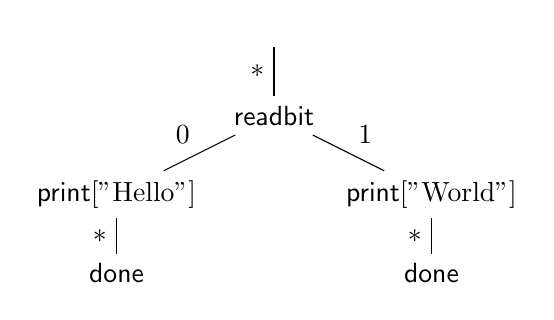
\begin{tikzpicture}
    \node (W) at (0,0) {};
    \node (R) at (0,-1) {$\kw{readbit}$};
    \node (W0) at (-2,-2) {$\kw{print}["\text{Hello}"]$};
    \node (W1) at (+2,-2) {$\kw{print}["\text{World}"]$};
    \node (K0) at (-2,-3) {$\kw{done}$};
    \node (K1) at (+2,-3) {$\kw{done}$};
    \path (W) edge node[auto,swap] {$*$} (R);
    \path (R) edge node[auto,swap] {0} (W0);
    \path (R) edge node[auto] {1} (W1);
    \path (W0) edge node[auto,swap] {$*$} (K0);
    \path (W1) edge node[auto,swap] {$*$} (K1);
  \end{tikzpicture}
\]
where we interpret edge labels
as moves of the environment,
and node labels as moves of the system.

%Terms are constructed by
%applying function symbols $e \in E$
%to subcomputations given for each $r \in \kw{ar}(e)$.
%In simple cases,
%the computation $e(x_r)_{r \in \kw{ar}(e)}$
%first triggers an effect $e$;
%then the context chooses $r$
%and resumes the computation as $x_r$.
%For example,
%the following effect signature
%models a very basic input/output facility:
%\[
%  E_\kw{io} :=
%    \{ \kw{readbit} : \mathbbm{2}, \:
%       \kw{writebit}[n] : \mathbbm{1} \mid
%       n \in \mathbbm{2} \}
%\]
%A computation which writes a zero,
%reads one bit, echoes its complement
%and continues as the computation $k$
%can be written as:
%\[
%  \kw{writebit}[0](
%    \kw{readbit}(
%      \kw{writebit}[1](k),
%      \kw{writebit}[0](k)))
%\]

%}}}

\subsection{Plays} \label{sec:intm:plays} %{{{

Building on these ideas,
we now introduce the partially ordered sets of plays
which we use to construct our specification monad.

\begin{definition}
The set $\bar{P}_E(A)$ of \emph{interactions}
for an effect signature $E$ and set of values $A$
is defined inductively:
\[
  s \in \bar{P}_E(A) ::=
    \underline{v} \mid
    \underline{m} \mid
    \underline{m} n s \,,
\]
where $v \in A$, $m \in E$ and $n \in \kw{ar}(m)$.
The set $\bar{P}_E(A)$ is ordered by the prefix relation
${\sqsubseteq} \subseteq \bar{P}_E(A) \times \bar{P}_E(A)$,
defined
as the smallest relation satisfying:
\[
  \underline{v} \sqsubseteq \underline{v} \,, \qquad
  \underline{m} \sqsubseteq \underline{m} \,, \qquad
  \underline{m} \sqsubseteq \underline{m} n t \,, \qquad
  \begin{prooftree}
    \hypo{s \sqsubseteq t}
    \infer1{\underline{m} n s \sqsubseteq \underline{m} n t}
  \end{prooftree} \,.
\]
\end{definition}

A play corresponds to a finite observation of
an interaction between the system and the environment.
At any point in such an interaction,
the system can terminate the interaction with a given value ($v$),
or it can trigger an effect $m \in E$ and
wait to be resumed by
an answer $n \in \kw{ar}(e)$ of the environment
($\underline{m} n s$).

A play which concludes before
the environment answers a query from the system ($\underline{m}$)
denotes that no information has been observed after that point.
It can be refined by a longer observation
of an interaction which begin with the same sequence of
questions and answers.
{\color{gray} Comment on the granularity?}

%}}}

\subsection{Interaction specifications} %{{{

We define our monad as the free distributive completion
of the corresponding poset of plays.

For the sake of conciseness and clarity,
we will use the order embedding associated with $\mathbf{FCD}$
implicitly,
so that an element of a poset $s \in P$
can also be regarded as an element of
its completion $s \in \mathbf{FCD}(P)$.
Likewise,
for a completely distributive lattice $L$,
we can implicitly
promote a monotonic operator
$f : P \rightarrow L$
to its extension
$f : \mathbf{FCD}(P) \rightarrow L$
as given by the universal property of
the free completely distributive lattice.
These conventions are at work
in the following definition.

\begin{definition} \label{def:intm} % Interaction specification monad {{{
The \emph{interaction specification monad}
for an effect signature $E$
maps a set of values $A$
to the free distributive completion
of the corresponding set of plays:
\[
    \mathcal{I}_E(A) :=
      \mathbf{FCD}(\bar{P}_E(A))
\]
An element $x \in \mathcal{I}_E(A)$ is called
an \emph{interaction specification}.

The monad's action on a function $f : A \rightarrow B$
replaces the values in
an interaction specification with their image by $f$:
\begin{align*}
  \mathcal{I}_E(f)(\underline{v}) &:= \underline{f(v)} \\
  \mathcal{I}_E(f)(\underline{m}) &:= \underline{m} \\
  \mathcal{I}_E(f)(\underline{m} n s) &:=
    \underline{m} n \, \mathcal{I}_E(f)(s) \,.
\end{align*}
The monad's unit
$\eta^E_A : A \rightarrow \mathcal{I}_E(A)$
is the embedding of a single play
consiting only of the given value:
\[
    \eta^E_A(v) := \underline{v}
\]
Finally, the multiplication
$\mu^E_A : \mathcal{I}_E(\mathcal{I}_E(A)) \rightarrow \mathcal{I}_E(A)$
carries out the outer computation and
sequences it with any computation it evaluates to:
\begin{align*}
  \mu^E_A(\underline{x}) &:= x \\
  \mu^E_A(\underline{m}) &:= \underline{m} \\
  \mu^E_A(\underline{m} n s) &:=
    \underline{m} \sqcup \underline{m} n \, \mu^E_A(s) \,.
\end{align*}

\begin{proof} %{{{
From the definitions above and
the fact that $\mathbf{FCD}$ is itself a monad,
it is straightforward to verify that
for all functions $f : A \rightarrow B$,
\[
    \eta^E_B \circ f = \mathcal{I}_E(f) \circ \eta^E_A \,.
\]
By inductions on plays, we can also show that:
\[
    \mu^E_B \circ \mathcal{I}_E(\mathcal{I}_E(f)) =
      \mathcal{I}_E(f) \circ \mu^E_A \,.
\]
This establishes that $\eta^E$ and $\mu^E$
are natural transformations.
By a similar approach,
we can show for a set $X$ that:
\begin{align*}
  \mu^E_X \circ \mathcal{I}_E(\mu^E_X) &=
    \mu^E_X \circ \mu^E_{\mathcal{I}_E(X)} \\
  \mu^E_X \circ \mathcal{I}_E(\eta^E_X) &=
    \mu^E_X \circ \eta^E_{\mathcal{I}_E(X)} \,,
\end{align*}
so that $\mathcal{I}_E$ is indeed a monad.
\end{proof}
%}}}
\end{definition}
%}}}

The most subtle aspect of Def.~\ref{def:intm}
is the case for $\mu^E_A(\underline{m} n s)$,
which includes $\underline{m}$ as well as $\underline{m} n \mu^E_A(s)$.
This is both
to ensure that the effects of the first computation are preserved
when the second computation is undefined, and
to ensure the monotonicity of the underlying function
used to define $\mu^E_A$.
Consider for example
$\underline{m} n \underline{\bot} \in \bar{P}_E(\mathcal{I}_E(A))$.
The $\mathbf{FCD}$ extension
of the function $s \mapsto \underline{m} n s$
preserves $\bot$,
with the consequence that
$\underline{m} = \mu^E_A(\underline{m}) \nsqsubseteq
 \underline{m} n \mu^E_A(\underline{\bot}) = \bot$,
even though
$\underline{m} \sqsubseteq \underline{m} n \underline{\bot}$.

As usual,
the Kleisli extension of a function $f : A \rightarrow \mathcal{I}_E(B)$
is the function $f^\dagger = \mu^E_B \circ \mathcal{I}_E(f)$.
Given directly:
\begin{align*}
  f^\dagger(\underline{v}) &:= f(v) \\
  f^\dagger(\underline{m}) &:= \underline{m} \\
  f^\dagger(\underline{m} n s) &:=
    \underline{m} \sqcup \underline{m} n f^\dagger(s)
\end{align*}

%}}}

\subsection{Basic constructions} %{{{

[Introduce the monadic notations and constructions
from the refinement calculus which we use in the rest
of the section]

\begin{color}{gray}

The refinement lattice over $\mathcal{I}_E(A)$
provides unbounded demonic choices
in the form of arbitrary meets
(realized as the union of the outer sets),
and unbounded angelic choices
in the form of arbitrary joins
(realized as the intersection of the outer sets).
A refinement $x \sqsubseteq y$ expresses that
$y$ offers fewer demonic choices and more angelic choices than $x$.

In particular,
the least element $\bot = \bigsqcup \varnothing$
corresponds to a situation where the environment has no choices
and the computation cannot be resumed.
It can be refined by any other computation and
we will use it to interpret undefined behaviors and silent divergence.
Conversely,
the greatest element $\top = \bigsqcap \varnothing$
corresponds to the \emph{magic} behavior
which refines all others:
the system has no choices,
therefore any behavior is vacuously satisfactory.

Another special case of angelic choice is
the \emph{assertion} of a proposition $P$,
which returns the trivial value $*$ if $P$ holds
and is equal to $\bot$ otherwise:
\[ \{P\} \in \mathcal{I}_E(\{*\}) :=
    \bigsqcup \{ \eta(*) \mid P \} \]
Dually,
the \emph{assumption} of $P$
is defined as follows,
and is equal to $\top$ when $P$ does not hold:
\[ [P] \in \mathcal{I}_E(\{*\}) :=
    \bigsqcap \{ \eta(*) \mid P \} \]

\end{color}

%}}}

\subsection{Interactions} %{{{

The operations of an effect signature $E$
can be promoted to interaction specifications of $\mathcal{I}_E$
as follows.

\begin{definition}[Interaction primitive]
For an effect signature $E$, a set $A$ and
an operation $m \in E$,
the interaction specification
$\mathbf{I}_E^m \in \mathcal{I}_E(\kw{ar}(m))$
is defined as:
\[
  \mathbf{I}_E^m :=
    \bigsqcup_{n \in \kw{ar}(m)} \underline{m} n \underline{n}
\]
If the context permits,
we can write $\mathbf{I}_E^m$ simply as $m$.
\end{definition}
Note that in the play $\underline{m} n \underline{n}$,
the first occurence of $n$ is the environment's answer,
whereas the second occurence is the value returned by $\mathbf{I}_E^m$.

To model effect handling,
we can use a family of interaction specifications
$(f^m)_{m \in F}$
to provide an interpretation $f^m \in \mathcal{I}_F(\kw{ar}(m))$
of each effect $m \in F$
in terms of another effect signature $E$.
This allows us to transform an interaction specification
$x \in \mathcal{I}_F(A)$ of $F$
into an interaction specification
$x[f]$ of $E$.

\begin{definition}[Interaction substitution]
Given the effect signatures $E, F$ and the set $A$,
for an interaction specification $x \in \mathcal{I}_F(A)$
and a family $(f^m)_{m \in E}$ with $f^m \in \mathcal{I}_E(\kw{ar}(m))$,
the \emph{interaction substitution} $x[f] \in \mathcal{I}_E(A)$
is defined by:
\begin{align*}
  \underline{v}[f] &:= \underline{v} \\
  \underline{m}[f] &:= f^m ; \bot \\
  \underline{m}ns[f] &:= r \leftarrow f^m ; \{r = n\} ; s[f] \,.
\end{align*}
\end{definition}

The outcome of the interaction specification is left unchanged,
but effects are replaced by their interpretation.
Whenever the interpretation produces an outcome $r$,
the matching plays of the original computation
are allowed to proceed accordingly.

%}}}

\subsection{Game semantics} %{{{

As presented so far,
the interaction specification monad
can be seen as an extension of the refinement calculus
able to model effectful computations
for a given signature.

We now shift our point of view to game semantics
and show how interaction substitutions
can be used to define a simple category of games and strategies
featuring dual nondeterminism and refinement.

\begin{definition}[Interaction substitutions as morphisms]
Consider the effect signatures $E$, $F$ and $G$.
We will write $f : E \rightarrow F$
whenever $(f^m)_{m \in F}$ is a family of interactive computations
such that $f^m \in \mathcal{I}_E(\kw{ar}(m))$.
Then for $f : E \rightarrow F$ and $g : F \rightarrow G$,
we define $g \circ f : E \rightarrow G$ as:
\[ (g \circ f)^m = f^m[g] \,. \]
The completely distributive lattice structure
of $\mathcal{I}_F(-)$ can be extended pointwise
to interaction substitutions,
so that for a family $(f_i)_{i \in I}$
with $f_i : E \rightarrow F$,
we can define the substitutions
$(\bigsqcup_{i \in I} f_i) : E \rightarrow F$ and
$(\bigsqcap_{i \in I} f_i) : E \rightarrow F$ as:
\begin{gather*}
    \left( \bigsqcup_{i \in I} f_i \right)^m :=
      \bigsqcup_{i \in I} f_i^m \qquad
    \left( \bigsqcap_{i \in I} f_i \right)^m :=
      \bigsqcap_{i \in I} f_i^m \,,
\end{gather*}
and for $f, g : E \rightarrow F$
we can define refinement as:
\[
    f \sqsubseteq g \: \Leftrightarrow \:
    \forall m \in F \bdot f^m \sqsubseteq g^m \,.
\]
\end{definition}

An interaction substitution $f : E \rightarrow F$
can be interpreted as a \emph{well-bracketed} strategy for the game
${!E} \multimap F$.
In this game,
the environment first plays a move $m \in F$.
The system can then ask a series of questions
$q_1, \ldots q_k \in E$
to which the environment will reply with
answers $r_i \in \kw{ar}(q_i)$,
and finally produce an answer $n \in \kw{ar}(m)$
to the environment's initial question $m$.
\begin{color}{gray}
The arena for ${!E} \multimap F$
can be described as:
\[
  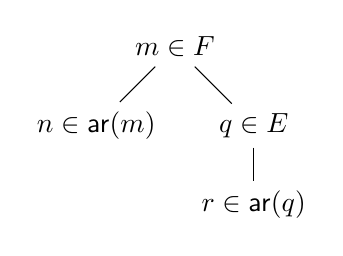
\begin{tikzpicture}
    %\node (S) at (0,3) {$\star$};
    \node (BQ) at (0,2) {$m \in F$};
    \node (BA) at (-1,1) {$n \in \kw{ar}(m)$};
    \node (AQ) at (+1,1) {$q \in E$};
    \node (AA) at (+1,0) {$r \in \kw{ar}(q)$};
    %\path (S) edge (BQ);
    \path (BQ) edge (BA);
    \path (BQ) edge (AQ);
    \path (AQ) edge (AA);
  \end{tikzpicture}
\]
\end{color}
The plays of ${!E} \multimap F$
are restricted to a single top-level question $m$.
In addition, the well-bracketing requirement
imposes that at any point,
only the most recent pending question
may be answered.

Our model extends the usual notion of strategy
by introducing demonic choice and
relaxing the environment determinacy constraint.
The definition of $g \circ f$ given above
otherwise corresponds to the traditional
definition of strategy composition.
The identity strategy is given by $\mathbf{I}_E : E \rightarrow E$.

\begin{lemma}
Consider the effect signatures $E, F, G, H$ and
the substitutions
$f : E \rightarrow F$,
$g : F \rightarrow G$ and
$h : G \rightarrow H$.
The following properties hold:
\begin{gather*}
  \mathbf{I}_F \circ f = f \circ \mathbf{I}_E = f \\
  h \circ (g \circ f) = (h \circ g) \circ f
\end{gather*}
Composition preserves all suprema on the left,
and all non-empty suprema on the right.
\begin{proof}
As before,
using the monadic properties of $\mathbf{FCD}$
and inductions on plays.
\end{proof}
\end{lemma}

Having established the relevant properties,
we can now define our first category of games and strategies.

\begin{definition}
The category $\gcat^{ib}$ has effect signatures as objects
and interaction substitutions as morphisms.
The hom-sets $\gcat^{ib}(E, F)$
are completely distributive lattices,
with composition preserving all suprema on the left,
and all non-empty suprema on the right.
\end{definition}

%}}}

\subsection{Products} %{{{

Effect signatures can be combined in the following way.

\begin{definition}
We define the effect signature
$\mathbf{1} := \varnothing$.
For a family of effect signatures $(E_i)_{i \in I}$,
we define:
\[
  \bigotimes_i E_i := \{ (i, e) : \kw{ar}(e) \mid i \in I, e \in E_i \}
\]
\end{definition}

For example,
the signature $E_\kw{io}$ above is equivalent
to the following composite one:
\[
    \{ \kw{readbit} : \mathbbm{2} \} \otimes
    \{ \kw{print}[s] : \mathbbm{1} \mid s \in \kw{string} \} \otimes
    \{ \kw{done} : \varnothing \}
\]

The construction $\otimes$ gives products in the category $\gcat^{ib}$,
as demonstrated below.

\begin{lemma}
The category $\gcat^{ib}$ has all products.
The corresponding objects are given by $\bigotimes_{i \in I} E_i$,
and the projection arrow
is given for each $i \in I$ as
the interaction substitution:
\begin{gather*}
    \pi_i : \bigotimes_{j \in I} E_j \rightarrow E_i \qquad
    \pi_i^m := (i, m) \,.
\end{gather*}
\begin{proof}
We need to show that for an effect signature $X$
and a collections of substitutions $(f_i)_{i \in I}$ with
$f_i : X \rightarrow E_i$,
there is a unique
$\langle f_i \rangle_{i \in I} : X \rightarrow \bigotimes_{i \in I} E_i$
such that for all $i \in I$:
\[
    f_i = \pi_i \circ \langle f_j \rangle_{j \in I} \,.
\]
Note that for $x : X \rightarrow \bigotimes_{i \in I} E_i$,
$i \in I$ and $m \in E_i$, we have:
\[
    (\pi_i \circ x)^m = \pi_i^m[x] = (i, m) [x] = x^{(i, m)}
\]
Hence, $\langle f_i \rangle_{i \in I}$ is uniquely defined as:
\[
    \langle f_i \rangle_{i \in I}^{(j, m)} := f_j^m \,.
\]
\end{proof}
\end{lemma}

%}}}

\subsection{Example: game semantics for CompCertO}

[Summarize the semantic model used in CompCertO
and show how to assign semantics to transition systems
as morphisms
$\llbracket L \rrbracket : \gcat^{ib}(\mathbb{E} \otimes A, B)$.

Ideally, express horizontal composition
in terms of the interaction specification monad]

%}}}

\section{Stateful and reentrant strategies} %{{{

% Preamble {{{

As we have shown,
the morphisms of $\gcat^{ib}(E, F)$
correspond to well-bracketed strategies
for the game ${!E} \multimap F$.
By the \emph{bang lemma} given in \cite{gamesem99},
they also corresponds to the
\emph{innocent} well-bracketed strategies
for the game ${!E} \multimap {!F}$.

That game proceeds similarly to ${!E} \multimap F$,
but instead of playing a single instance of $F$,
the environment is free to instantiate a new instance
whenever it is in control,
by asking a new top-level question $m \in F$.
The system's own questions in ${!E}$
are made in the context of a specific question in ${!F}$;
this information is often encoded using \emph{justification pointer},
whereby all non-top-level moves are required to refer to
an earlier move,
in a way that is compatible with the enabling relation
used to define the game's arena.
The well-bracketing condition only allows the players
to answer the most recent pending question.
In our limited setting,
the innocence condition requires that the system
behave in the same way for each top-level question.

To specify an innocent strategy
for our game ${!E} \multimap {!F}$,
it is enough to specify its behavior
for a single question of $F$:
the behavior of the full strategy can be reconstructed
by duplicating this behavior whenever needed.
This is traditionally expressed as a promotion operator
mapping a strategy $\sigma : {!A} \multimap B$
to the strategy $\sigma^\dagger : {!A} \multimap {!B}$.

%}}}

\subsection{Overview} %{{{
\label{sec:arrow}

In the game ${!E} \multimap {!F}$,
when the system asks a quetion in ${!E}$,
the environment may delay its answer
and instead ask a new question of its own in ${!F}$.
Since we only consider well-bracketed strategies,
such ``reentrant'' questions must be answered by the system
before then environment can answer the original one.

More generally,
the well-bracketing requirement
enforces a kind of \emph{stack discipline}
on the succession of questions and answers.
A well-bracketed play
can be interpreted as an activation tree,
where questions are understood as function calls
between the system and the environment,
and answers to a question are understood as the
corresponding function call returning.
The stack discipline is enforced by the fact that
questions must be answered in the reverse order
in which they were asked.
The alternation constraint
corresponds to the sequential nature of the computation.

%}}}

\subsection{Games} %{{{

To facilitate reasoning,
and make it easier to describe operators on strategies
in a systematic way,
we describe games as a specific kind of graph
where vertices represent players
and eges represent questions that can be asked
by one player to another.
%Operations on plays and strategies
%can then be specified in terms of
%their action on individual questions.
Generalizing from effect signatures,
questions are assigned an arity
which gives the type of the answer.

\begin{definition}
A \emph{game signature} $\Gamma$
is a set of players with a distinguished element $\kw{O}$,
together with an effect signature $\Gamma(u, v)$
for all $u, v \in \Gamma$.
The operations $m \in \Gamma(u, v)$ are called
the \emph{questions} of $u$ to $v$,
and the elements $n \in \kw{ar}(m)$ are called
\emph{answers} to the question $m$.
\end{definition}

We will depict game signatures as directed graphs
whose vertices are the players and
whose edges are labelled by the corresponding signature.
Missing edges correspond to the empty signature $\varnothing$.
For example,
%an effect signature $E$ corresponds to
%the single-player game signature:
%\[
%  [E] =
%  \begin{tikzpicture}[baseline=(O.base)]
%    \node[circle,double,draw] (O) at (0,0) {$\kw{O}$};
%    \path[->] (O) edge[loop right] node[auto] {E} (O);
%  \end{tikzpicture} \,,
%\]
%and
the game ${!E} \multimap {!F}$ will be generated by
the game signature:
\[
  [E,F] =
  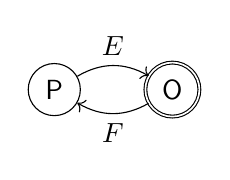
\begin{tikzpicture}[baseline=(O.base),scale=1.5]
    \node[circle,draw,double] (O) at (0,0) {$\kw{O}$};
    \node[circle,draw] (P) at (-1,0) {$\kw{P}$};
    \path[->] (P) edge[bend left] node[above] {$E$} (O);
    \path[->] (O) edge[bend left] node[below] {$F$} (P);
  \end{tikzpicture}
\]

Game signatures with more than two players
can be convenient to describe composite systems.
For instance,
consider the composition $\tau \circ \sigma$ of
the strategy $\sigma : {!E} \multimap {!F}$ and
the strategy $\tau : {!F} \multimap {!G}$.
Questions of the environment are directed to $\tau$,
questions of $\tau$ are directed to $\sigma$,
and questions of $\sigma$ are directed back to the environment.
This is described by the following three-player game signature:
\[
  [E,F,G] =
  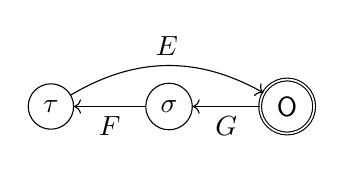
\begin{tikzpicture}[baseline=(O.base),scale=1.5]
    \node[circle,double,draw] (O) at (1,0) {$\kw{O}$};
    \node[circle,draw] (P2) at (0,0) {$\sigma$};
    \node[circle,draw] (P1) at (-1,0) {$\tau$};
    \path[->] (O) edge node[below] {$G$} (P2);
    \path[->] (P2) edge node[below] {$F$} (P1);
    \path[->] (P1) edge[bend left] node[above] {$E$} (O);
  \end{tikzpicture}
\]
When we consider the ways in which questions propagate
through a system such as the one above,
the distinguished player $\kw{O}$ serves the role
of both a source and sink.
As such, it is visually useful
to depict $\kw{O}$ as two nodes,
one capturing the incoming edges of $\kw{O}$, and
one capturing its outgoing edges:
\begin{gather*}
  [E,F] =
  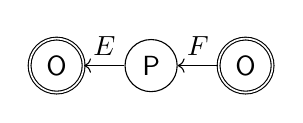
\begin{tikzpicture}[baseline=(O1.base),scale=1.2]
    \node[circle,double,draw] (O1) at (1,0) {$\kw{O}$};
    \node[circle,draw] (P) at (0,0) {$\kw{P}$};
    \node[circle,double,draw] (O2) at (-1,0) {$\kw{O}$};
    \path[->] (O1) edge node[above] {$F$} (P);
    \path[->] (P) edge node[above] {$E$} (O2);
  \end{tikzpicture} \\
  [E,F,G] =
  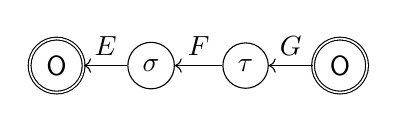
\begin{tikzpicture}[baseline=(O1.base),scale=1.2]
    \node[circle,double,draw] (O1) at (0,0) {$\kw{O}$};
    \node[circle,draw] (P1) at (-1,0) {$\tau$};
    \node[circle,draw] (P2) at (-2,0) {$\sigma$};
    \node[circle,double,draw] (O2) at (-3,0) {$\kw{O}$};
    \path[->] (O1) edge node[above] {$G$} (P1);
    \path[->] (P1) edge node[above] {$F$} (P2);
    \path[->] (P2) edge node[above] {$E$} (O2);
  \end{tikzpicture}
\end{gather*}

As another example of a game signature,
a situation where
$\sigma_1 : E_1 \rightarrow F_1$ and
$\sigma_2 : E_2 \rightarrow F_2$
interact with the environment
independently of one another
can be described as:
\[
  [E_1,F_1] \vee [E_2,F_2] =
  \begin{tikzpicture}[baseline=(O.base),xscale=1.2]
    \node[circle,draw,double] (O1) at (+1,0) {$\kw{O}$};
    \node[circle,draw,double] (O2) at (-1,0) {$\kw{O}$};
    \node[circle,draw] (P1) at (0,+0.5) {$\sigma_1$};
    \node[circle,draw] (P2) at (0,-0.5) {$\sigma_2$};
    \path[->] (O1) edge node[auto=right] {$F_1$} (P1);
    \path[->] (P1) edge node[auto=right] {$E_1$} (O2);
    \path[->] (O1) edge node[auto=left] {$F_2$} (P2);
    \path[->] (P2) edge node[auto=left] {$E_2$} (O2);
  \end{tikzpicture}
\]
The signature above will be used to compute
tensor products of strategies.
These constructions generalize as follows.

\begin{definition}[Constructions on game signatures]
For a collection of effect signature $(E_i)_{1 \le i \le n}$
and an effect signature $F$,
the game signature $[ E_1, \ldots, E_n, F ]$
has the players
$\kw{O}, \kw{P}_1, \ldots, \kw{P}_n$
and the following edges:
\[
  [E_1, \ldots, E_n, F] :=
  \begin{tikzpicture}[scale=1.2,baseline=(O.base)]
    \node[circle,draw,double] (O1) at (0,0) {$\kw{O}$};
    \node[circle,draw] (P1) at (1,0) {$\kw{P}_1$};
    \node (D) at (2,0) {$\ldots$};
    \node[circle,draw] (Pn) at (3,0) {$\kw{P}_n$};
    \node[circle,draw,double] (O2) at (4,0) {$\kw{O}$};
    \path[->] (P1) edge node[above] {$E_1$} (O1);
    \path[->] (D) edge node[above] {$E_2$} (P1);
    \path[->] (Pn) edge node[above] {$E_n$} (D);
    \path[->] (O2) edge node[above] {$F$} (Pn);
  \end{tikzpicture}
\]
For a collection of game signatures $(\Gamma_i)_{i \in I}$,
the \emph{wedge sum} $\bigvee_{i \in I} \Gamma_i$ has the players:
\[
    \{ \kw{O} \} \cup
    \{ (i, p) \mid i \in I \wedge p \in \Gamma_i \setminus \{ \kw{O} \} \}
\]
For $i \in I$ and $p \in \Gamma_i$, the corresponding player in
$\bigvee_{j \in I} \Gamma_j$ is:
\[
  \iota_i(p) := \begin{cases}
    \kw{O} & \text{if } p = \kw{O} \\
    (i, p) & \text{otherwise.}
  \end{cases}
\]
Then for each question $m : u \rightarrow v$ in $\Gamma_i$,
the wedge sum has a corresponding question
$\iota_i(m) : \iota_i(u) \rightarrow \iota_i(v)$.
\end{definition}

Note that the empty game signature $0$ can be
described in the following way:
\[
  0 := \bigvee \varnothing =
  \begin{tikzpicture}[baseline=(O.base)]
    \node[circle,draw,double] {$\kw{O}$};
  \end{tikzpicture}
\]

%}}}

\subsection{Plays and strategies} %{{{

The description of the game ${!E} \multimap {!F}$
using the game signature $[E, F]$
already encodes the alternating aspect of plays.
For the purpose of constructing well-bracketed plays,
a path in a simple game
can be understood as a stack of pending questions.
The well-bracketed plays over a game signature
can be described as follows.

\begin{definition}[Well-bracketed plays]
The \emph{balanced plays}
starting at each player in
a game signature $\Gamma$
are given
as the family of sets
$(\hat{P}_\Gamma^u)_{u \in \Gamma}$
defined inductively by the rules:
\[
  \epsilon \in \hat{P}_\Gamma^u
  \qquad
  \begin{prooftree}
    \hypo{s \in \hat{P}_\Gamma^u}
    \hypo{m \in \Gamma(u, v)}
    \hypo{t \in \hat{P}_\Gamma^v}
    \hypo{n \in \kw{ar}(m)}
    \infer4{smtn \in \hat{P}_\Gamma^u}
  \end{prooftree}
\]
The \emph{well-bracketed plays}
from one player to another
are given as the family of sets
$(P_\Gamma^{u,v})_{u,v \in \Gamma}$
defined by:
\[
  \begin{prooftree}
    \hypo{s \in \hat{P}_\Gamma^u}
    \infer1{s \in P_\Gamma^{u,u}}
  \end{prooftree}
  \qquad
  \begin{prooftree}
    \hypo{s \in \hat{P}_\Gamma^u}
    \hypo{m \in \Gamma(u, v)}
    \hypo{t \in P_\Gamma^{v,w}}
    \infer3{smt \in P_\Gamma^{u,w}}
  \end{prooftree}
\]
\end{definition}

This direct definition of well-bracketed plays
is similar to the one given in \cite{mwjava}.
To define strategies,
we will consider in particular the plays
starting and ending at player $\kw{O}$.

\begin{definition}[Plays and strategies over a game signature]
The well-bracketed plays over a game signature $\Gamma$
are ordered under the prefix relation
defined by the rules:
\[
  \epsilon \sqsubseteq s \sqsubseteq smt \sqsubseteq smtn
  \qquad \qquad
  \begin{prooftree}
    \hypo{t \sqsubseteq t'}
    \infer1{smt \sqsubseteq smt'}
  \end{prooftree} \,.
\]
We will write
$P \, \Gamma := \langle P_\Gamma^{\kw{O},\kw{O}}, {\sqsubseteq} \rangle$
for the poset of plays over $\Gamma$.
The \emph{strategy specifications} for $\Gamma$
are given by its completion:
\[
    S \, \Gamma := \mathbf{FCD}(P \, \Gamma) \,.
\]
\end{definition}

%}}}

\subsection{Operators} %{{{

The strategy specifications we have described
are fairly complex mathematical objects,
Because of this, it is challenging to
define and reason about operators
directly at this level.
Fortunately,
game signatures provide us with a systematic way
of describing operators on stratgies.
The action
$\Gamma[\kw{P_1} := \sigma_1, \ldots, \kw{P_n} := \sigma_n]$
of a game signature $\Gamma$ with players
$\kw{O}, \kw{P}_1, \ldots \kw{P}_n$
on the strategies
$\sigma_1, \ldots, \sigma_n$
is obtained by playing the strategies
against each other as each of the players
in the game corresponding to $\Gamma$,
with $\kw{O}$ representing the environment
of the resulting system.
We will show that operators can be combined
at the level of game signatures,
allowing us to describe and reason about their interactions
in a systematic way
and with as little ``administrative'' overhead as possible.

To illustrate this method,
we use the composition of strategies as an example.
The traditional definition of composition
in categories of games and strategies,
as given for example in \cite{gamesem99},
is as follows.
The strategy $\sigma : A \rightarrow B$,
plays the game $B$ as the proponent
and the game $A$ as the opponent.
The strategy $\tau : B \rightarrow C$,
plays the game $C$ as the proponent
and the game $B$ as the opponent.
Their composition $\tau \circ \sigma : A \rightarrow C$
is obtained by first considering \emph{interaction sequences}
in a game consisting of the three components $A, B, C$.
Given such a sequence $s \in P_{A,B,C}$,
we can project out
a play $s \restriction A,B$ for the game $A \rightarrow B$,
a play $s \restriction B,C$ for the game $B \rightarrow C$, and
a play $s \restriction A,C$ for the game $A \rightarrow C$.
The composite strategy $\tau \circ \sigma$
can then be given as the set of plays:
\[
    \{ (s \restriction A,C) \mid
       s \in P_{A,B,C} \wedge
       (s \restriction A,B) \in \sigma \wedge
       (s \restriction B,C) \in \tau \} \,.
\]

In our setting,
composition is entirely described by
the three-player game signature $[A,B,C]$.
The plays for this game signature
correspond to the interaction sequences $s \in P_{A,B,C}$.
The projections correspond to the views
of the interaction for each of the players.
These projections will be defined as
transformations of the following kind.

\begin{definition}
A \emph{transformation}
from the game signature $\Gamma_1$
to the game signature $\Gamma_2$
associates to each player $p \in \Gamma_1$ a player $f(p) \in \Gamma_2$
with $f(\kw{O}) = \kw{O}$,
and to each question $m \in \Gamma_1(u,v)$
a \emph{path} of questions in $\Gamma_2$:
\[
  f(u) = p_0 \xrightarrow{m_1'} p_1 \xrightarrow{m_2'} \cdots
             \xrightarrow{m_n'} p_n = f(v) \,,
\]
written as
$f(m) = m_1' m_2' \cdots m_n' : f(u) \twoheadrightarrow f(v)$, and
such that
$\kw{ar}(m_1') = \cdots = \kw{ar}(m_n') = \kw{ar}(m)$.
We extend $f$ itself to the paths in $\Gamma_1$
by taking the image of $m_1 \cdots m_n : u \twoheadrightarrow v$
to be:
\[
  f(m_1 \cdots m_n) := f(m_1) \cdots f(m_n) :
    f(u) \twoheadrightarrow f(v) \,.
\]
In other words,
a transformation
is a structure-preserving map on paths.
We write $\mathbf{GST}$ for the category of
game signatures and transformations.
\end{definition}

When composing the strategy specifications
$\sigma \in S \, [E, F]$ and
$\tau \in S \, [F, G]$
to obtain $\tau \circ \sigma \in S \, [E, F]$,
we will use the transformation
$\psi^c_X : [E,F,G] \rightarrow [E,G]$
to describe the externally observable behavior
of the game $[E,F,G]$:
\begin{gather*}
  \psi^c_X :
  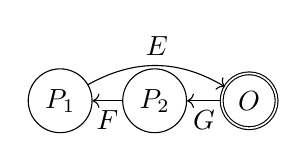
\begin{tikzpicture}[baseline=(O.base),scale=1.2]
    \node[circle,double,draw] (O) at (1,0) {$O$};
    \node[circle,draw] (P2) at (0,0) {$P_2$};
    \node[circle,draw] (P1) at (-1,0) {$P_1$};
    \path[->] (O) edge node[below] {$G$} (P2);
    \path[->] (P2) edge node[below] {$F$} (P1);
    \path[->] (P1) edge[bend left] node[above] {$E$} (O);
  \end{tikzpicture}
  \rightarrow
  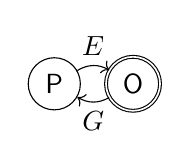
\begin{tikzpicture}[baseline=(O.base)]
    \node[circle,draw,double] (O) at (0,0) {$\kw{O}$};
    \node[circle,draw] (P) at (-1,0) {$\kw{P}$};
    \path[->] (P) edge[bend left] node[above] {$E$} (O);
    \path[->] (O) edge[bend left] node[below] {$G$} (P);
  \end{tikzpicture}
  \\
  \psi^c_X(\kw{P}_1) = \psi^c_X(\kw{P}_2) = \kw{P} \qquad
  \psi^c_X(\kw{O}) = \kw{O}
  \\
  \psi^c_X(m) = \begin{cases}
    \epsilon & \text{if } m \in F \\
    m & \text{otherwise}
  \end{cases}
\end{gather*}
This can be described concisely as
$\psi^c_X = [\mathrm{id}, \epsilon, \mathrm{id}]$,
with:
\begin{align*}
  \psi^c_1 &:= [\mathrm{id}, \mathrm{id}, \epsilon] :
    [E,F,G] \rightarrow [E,F] \\
  \psi^c_2 &:= [\epsilon, \mathrm{id}, \mathrm{id}] :
     [E,F,G] \rightarrow [F,G]
\end{align*}
defined similarly.
These transformations can then be extended to plays
to obtain our version of the projections $(s \restriction X,Y)$.

\begin{definition}[Action on plays]
A transformation
$f : \Gamma_1 \rightarrow \Gamma_2$
can be extended to a monotonic function on plays
$P f  : P \, {\Gamma}_1 \rightarrow P \, {\Gamma}_2$.
We define:
\begin{align*}
  P f (\epsilon) &= \epsilon \\
  P f (smt) &= P f (s) \cdot f(m) \cdot P f (t) \\
  P f (smtn) &= P f (s) \cdot f(m) \cdot P f (t) \cdot n^{|f(m)|} \,,
\end{align*}
where $n^{|f(m)|}$ denotes a sequence $nn \cdots n$
of copies of the answer $n \in \kw{ar}(m)$
of same length as the path $f(m)$.
\end{definition}

We can now formulate the composition of strategy specifications as follows.
The ``footprint'' of the plays $s_1 \in P \, [E,F]$ and $s_2 \in P \, [F,G]$
can be defined as:
\[
  \psi^c(s_1, s_2) :=
    \bigsqcup_{s \in P [E,F,G]}
    \{ \psi^c_1(s) \sqsubseteq s_1 \wedge \psi^c_2(s) \sqsubseteq s_2 \} ;
    \psi^c_X(s) \,.
\]
In other words,
the angel chooses a global play $s$
matching $s_1$ and $s_2$
and produces its external view.
By extending $\psi^c$ to strategy specifications
in the expected way, we obtain:
\[
  \tau \circ \sigma = 
    s \leftarrow \sigma ;
    t \leftarrow \tau ;
    \psi^c(s, t) \,.
\]

The following definition
generalizes this approach to arbitrary game signatures.

\begin{definition}[Operators]
The \emph{indegree} and \emph{outdegree}
of a player $p$ in a game signature $\Gamma$
are the effect signatures:
\[
  \Gamma_p^- := \bigotimes_{u \in \Gamma} \Gamma(u, p)
  \qquad
  \Gamma_p^+ := \bigotimes_{v \in \Gamma} \Gamma(p, v)
\]
For a question $m : u \rightarrow v$ in $\Gamma$,
we write its $\emph{incoming}$ and $\emph{outgoing traces}$
for player $p \in \Gamma$ as:
\begin{gather*}
  \check{\pi}_p(m) = \begin{cases}
    m & \text{if } v = p \\
    \epsilon & \text{otherwise}
  \end{cases}
  \quad
  \hat{\pi}_p(m) = \begin{cases}
    m & \text{if } u = p \\
    \epsilon & \text{otherwise}
  \end{cases}
\end{gather*}
Then the \emph{internal projections} of $\Gamma$
are defined by the transformations
$\pi_p : \Gamma \rightarrow [ \Gamma_p^+, \Gamma_p^- ]$
which map the player $u \in \Gamma$
and the question $m : u \rightarrow v$ to:
\[
  \pi_p(u) := \begin{cases}
    \kw{P} & \text{if } u = p \\
    \kw{O} & \text{otherwise}
  \end{cases}
  \quad
  \pi_i(m) :=
    \check{\pi}_p(m) \cdot \hat{\pi}_p(m) \,,
\]
and the \emph{external projection}
is defined by the transformation
$\bar{\pi}_p : \Gamma \rightarrow [ \Gamma_p^-, \Gamma_p^+ ]$
which maps $u \in \Gamma$
and $m : u \rightarrow v$ to:
\[
  \bar{\pi}_p(u) := \begin{cases}
    \kw{O} & \text{if } u = p \\
    \kw{P} & \text{otherwise}
  \end{cases}
  \quad
  \bar{\pi}_p(m) :=
    \hat{\pi}_p(m) \cdot \check{\pi}_p(m) \,.
\]
The \emph{action} of a game signature $\Gamma$
with players $\kw{O}, \kw{P}_1, \ldots \kw{P}_n$
on the strategies
$\sigma_i \in S \, [\Gamma_{\kw{P}_i}^+, \Gamma_{\kw{P}_i}^-]$
yields the strategy:
\[
  \Gamma[\kw{P}_i := \sigma_1]_{1 \le i \le n} \in
    S \, [\Gamma_\kw{O}^-, \Gamma_\kw{O}^+] \,,
\]
defined as:
\[
  s_1 \leftarrow \sigma_1 ; \cdots ; s_n \leftarrow \sigma_n ; 
    \bigsqcup_{s \in P \Gamma}
    \{ \forall i \bdot \pi_{\kw{P}_i}(s) \sqsubseteq s_i \} ;
    \bar{\pi}_\kw{O}(s) \,.
\]
\end{definition}

In the case of $\Gamma = [E, F, G]$,
the internal and external projections correspond
to the transormations $\psi^c_i$ and $\psi^c_X$,
up to the appropriate isomorphisms
between $\Gamma^+_p, \Gamma^-_p$ and $E, F, G$.
Therefore,
the interactive composition of strategies
can be described as:
\[
  \tau \circ \sigma \cong
    [E, F, G][\kw{P}_1 :\cong \tau, \kw{P}_2 :\cong \sigma] \,.
\]

Compositions of operators
described by game signatures
can themselves be characterized
in terms of game signatures.
In the composite signature
$\Gamma[\kw{P}_i := \Gamma_i]_{1 \le i \le n}$,
each player $\kw{P}_i \in \Gamma$
is replaced by a subgraph derived from
the signature $\Gamma_i$.
The indegree $\Gamma^-_{\kw{P}_i}$ in $\Gamma$
is identified with the outdegree $\Gamma^+_{i, \kw{O}}$ in $\Gamma_i$,
and conversely
the outdegree $\Gamma^+_{\kw{P}_i}$
is identified with the indegree $\Gamma^-_{i, \kw{O}}$.

For example,
[show diagrams for the associativity of composition
and identity].

In the general case,
the operator composition of game signatures
can be described as follows.

\begin{definition}[Composition of game signatures]
For the game signatures $\Gamma$
and $(\Gamma_p)_{p \in \Gamma \setminus \kw{O}}$,
and the families of isomorphisms
$(f^+_p, f^-_p)_{p \in \Gamma \setminus \kw{O}}$
where:
\begin{align*}
    f_p^+ : \Gamma_p^-(\kw{O}) &\cong \Gamma^+(p)
    \\
    f_p^- : \Gamma_p^+(\kw{O}) &\cong \Gamma^-(p) \,,
\end{align*}
the composite game signature
$\Psi = \Gamma[p := \Gamma_p]_{p \in \Gamma \setminus \kw{O}}$
has a player $\kw{O}$ and a player $(p, p')$ for
each player $p \in \Gamma \setminus \{\kw{O}\}$ and
each $p' \in \Gamma_p \setminus \{\kw{O}\}$.
For convenience
we define $\Gamma_\kw{O} := [\Gamma_\kw{O}^-, \Gamma_\kw{O}^+]$.
Then the players of $\Psi$ are described by the set:
\[
  \sum_{p \in \Gamma} \Gamma_p \setminus \{\kw{O}\} \,,
\]
with $(\kw{O}, \kw{P})$ corresponding to the
$\kw{O}$ player of $\Psi$.
A question in $\Psi((u, u'), (v, v'))$
will be specified by
a question \emph{path} in $\Gamma$:
\[
  u = u_0 \xrightarrow{m_1}
      u_1 \xrightarrow{m_2}
      \cdots \xrightarrow{m_n}
      u_n = v
  \quad
  (m_i \in \Gamma(u_{i-1}, u_i))
\]
together with a question of $\Gamma_{u_i}$ for each $0 \le i \le n$:
\begin{itemize}
\item a question $m'_0 \in \Gamma_u(u', \kw{O})$,
\item a question $m'_i \in \Gamma_{u_i}(\kw{O}, \kw{O})$ for each $1 \le i < n$, and
\item a question $m'_n \in \Gamma_v(\kw{O}, v')$.
\end{itemize}
We will write:
\begin{align*}
  (u, u') = u^- \xrightarrow{m'_0} u^+
          \xrightarrow{m_1} u_1^-
          \xrightarrow{m'_1} u_1^+
         &\xrightarrow{m_2} u_2^-
          \xrightarrow{m'_2} \cdots \\ \cdots
          \xrightarrow{m_{n-1}} u_{n-1}^-
          \xrightarrow{m'_{n-1}} u_{n-1}^+
          \xrightarrow{m_{n}} v^-
         &\xrightarrow{m'_n} v^+ = (v, v') \,.
\end{align*}
We further require that for all $1 \le i \le n$:
\[ f^+_{u_{i-1}}(m'_{i-1}) = m_i =
   f^-_u(m'_{i}) \,, \]
so that all of the questions in the path
are the same up to the specified isomorphisms.
The questions of $\Psi((u, u'), (v, v'))$
are paths of the form above meeting this requirement
and are assigned arity
$\kw{ar}(m'_0) = \kw{ar}(m_1) = \cdots = \kw{ar}(m_n) = \kw{ar}(m'_n)$.
\end{definition}

[Some commentary]

\begin{lemma}

If
\[
  \sigma_p := \Gamma_p[p' := \sigma_{p,p'}]
\]
then:
\[
  \Psi[p := \Gamma_p][(p, p') := \sigma_{p, p'}] =
  \Psi[p := \sigma_p] \,.
\]
\end{lemma}

%}}}

---

OLD THINGS BELOW.

\begin{definition}
An \emph{operator} $\psi$ of arity $n$
from a family of game signature $(\Gamma_i)_{1 \le i \le n}$
to a game signature $\Gamma_X$
is given by:
\begin{itemize}
\item A game signature $\Gamma_G$ called the \emph{global signature};
\item An \emph{external view} $\psi_X : \Gamma_G \rightarrow \Gamma_X$;
\item An \emph{internal view} $\psi_i : \Gamma_G \rightarrow \Gamma_i$
  for each $1 \le i \le n$.
\end{itemize}
The image of the plays $(s_i)_{1 \le i \le n}$
where $s_i \in P \, {\Gamma_i}$
is given by:
\[
  \psi(s_1, \ldots, s_n) :=
    \bigsqcup_{s \in P \, {\Gamma_G}}
    \{ \forall i \bdot \psi_i(s) \sqsubseteq s_i \} ;
    \psi_X(s) \,.
\]
Then the action of $\psi$ on strategies is given by:
\[
  \psi(\sigma_1, \ldots, \sigma_n) :=
    s_1 \leftarrow \sigma_1 \, ; \, {\cdots} \, ; \,
    s_n \leftarrow \sigma_n \, ; \,
    \psi(s_1, \ldots, s_n) \,.
\]
\end{definition}

%}}}

\begin{color}{red}
WAIT A MINUTE.
Our game signatures already have all the needed information
to define operators on their own!

For an $n+1$-players game signature $\Gamma$,
we obtain an $n$-ary operator
with arguments:
\[
    \sigma_i : \bigotimes_{p \in \Gamma} \Gamma(\kw{P}_i, p) \rightarrow
               \bigotimes_{p \in \Gamma} \Gamma(p, \kw{P}_i)
\]
with the result:
\[
    \Gamma[\kw{P}_1 := \sigma_1, \ldots, \kw{P}_n := \sigma_n] :
    \bigotimes_{p \in \Gamma} \Gamma(p, \kw{O}) \rightarrow
    \bigotimes_{p \in \Gamma} \Gamma(\kw{O}, p)
\]
To compute it,
we apply the same principle as above.

These operators compose like butter:
we replace the node $\kw{P}_i$ with $\Sigma_i$ in $\Gamma$
to obtain $\Gamma \circ \langle \Sigma_1, \ldots , \Sigma_n \rangle$;
the incoming edge of $\kw{P}_i$ in $\Gamma$
correspond to the outgoing edges of $\kw{O}$ in $\Sigma_i$
and vice versa.
The the dreaded associativity proof becomes a simple
graphical thing, where we show that:
\begin{align*}
    [E,F,G,H] &= [E,F,H] \circ \langle [E,F], [F,G,H] \rangle \\
              &= [E,G,H] \circ \langle [E,F,G], [G,H] \rangle
\end{align*}
The operators of interest can all be described this way,
with
\begin{itemize}
\item identity strategy: $[E]$
\item identity operator: $[E,F]$
\item composition : $[E,F,G]$
\item tensor product : $[E,F] \vee [G,H]$
\item self-interaction :
  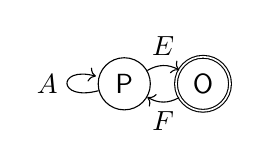
\begin{tikzpicture}[baseline=(O.base)]
    \node[circle,draw] (P) at (-1,0) {$\kw{P}$};
    \node[circle,draw,double] (O) at (0,0) {$\kw{O}$};
    \path[->] (P) edge[loop left] node[auto] {$A$} (P);
    \path[->] (P) edge[bend left] node[above] {$E$} (O);
    \path[->] (O) edge[bend left] node[below] {$F$} (P);
  \end{tikzpicture}
\end{itemize}

\end{color}

\subsection{Identity and composition} %{{{

Identity is defined as a nullary operator
$\mathrm{id}_E : 1 \rightarrow [E,E]$
with global signature $[E]$:
\begin{gather*}
  \mathrm{id}_E^X :
  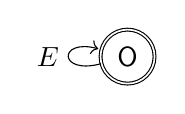
\begin{tikzpicture}[baseline=(O.base)]
    \node[circle,draw,double] (O) at (0,0) {$\kw{O}$};
    \path[->] (O) edge[loop left] node[auto] {$E$} (O);
  \end{tikzpicture}
  \Rightarrow
  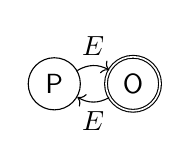
\begin{tikzpicture}[baseline=(O.base)]
    \node[circle,draw,double] (O) at (1,0) {$\kw{O}$};
    \node[circle,draw] (P) at (0,0) {$\kw{P}$};
    \path[->] (O) edge[bend left] node[below] {$E$} (P);
    \path[->] (P) edge[bend left] node[above] {$E$} (O);
  \end{tikzpicture}
  \\
  \mathrm{id}_E^X(\kw{O}) := \kw{O}
  \qquad
  \mathrm{id}_E^X(m) := mm
\end{gather*}
The definition of composition has been given above.

%}}}

\subsection{Monoidal structure} %{{{

We define the tensor product of strategies
as the operator
$\psi^{\otimes} : [E_1,F_1] \times [E_2,F_2] \rightarrow
 [E_1 \otimes E_2, F_1 \otimes F_2]$
with global plays in
$[E_1,F_1] \vee [E_2,F_2]$.

%}}}

\subsection{Self-interaction} %{{{

%}}}



---

[The basic idea is that we define
mappings between the players and edges of game signatures,
so that an edge of the first game maps to a path between
the corresponding players of the second game.
An operator of arity $n$ can be defined by two such mappings:
\[ \Gamma_I \Leftarrow \Gamma_G \Rightarrow \Gamma_X \,, \]
where $\Gamma_I = \Gamma_1 \vee \cdots \vee \Gamma_n$ is the \emph{internal} view,
$\Gamma_G$ is the \emph{global} view,
and $\Gamma_X$ is the \emph{external} view.
The internal view is a wedge sum
$\Gamma_1 \vee \cdots \vee \Gamma_n$
where the $n$ strategies we want to operate on
will play.
The mapping $\Gamma_I \Leftarrow \Gamma_G$
will determine which global plays correspond
to which interactions of the $n$ strategies
(allowing us to synchronize their moves),
and the mapping $\Gamma_G \Rightarrow \Gamma_X$
gives the result.
This works to define all that we want:
\begin{itemize}
\item Identity: $0 \Leftarrow [E] \Rightarrow [E,E]$
\item Composition: $[E,F] \vee [F,G] \Leftarrow [E,F,G] \Rightarrow [E,G]$
\item Tensor: \[ [E,F] \vee [G,H] \Leftarrow [E,F] \vee [G,H] \Rightarrow
  [E \otimes G, F \otimes H] \]
\item The $\kw{Z}$ operator for self-interaction:
  \[ [E \otimes A, A \otimes F] \Leftarrow
  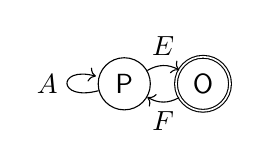
\begin{tikzpicture}[baseline=(O.base)]
    \node[circle,draw] (P) at (-1,0) {$\kw{P}$};
    \node[circle,draw,double] (O) at (0,0) {$\kw{O}$};
    \path[->] (P) edge[loop left] node[auto] {$A$} (P);
    \path[->] (P) edge[bend left] node[above] {$E$} (O);
    \path[->] (O) edge[bend left] node[below] {$F$} (P);
  \end{tikzpicture} \Rightarrow [E,F] \]
\end{itemize}
Then we can reason on operators by reasoning at the level of moves
in game signature mappings,
rather than having to handle the complicated
plays and strategies generated from them
directly.]

---

At the level of strategies the mapping
$\Gamma_I \Leftarrow \Gamma_G$ preserved joins
and so has a Galois adjoint $\Gamma_I \Leftarrow \Gamma_G$,
which allows us to compose with $\Gamma_G \Rightarrow \Gamma_X$
to build the overall operator on strategies.

\begin{definition}
A \emph{quiver homomorphism} from $Q_1$ to $Q_2$
as a function $f : Q_1 \rightarrow Q_2$ together with,
for each pair of vertices $u, v \in Q$,
a function $f_{u,v} : Q_1(u, v) \rightarrow Q_2(f(u), f(v))$
\end{definition}

\begin{definition}
A \emph{homomorphism of game signatures} $f : \Gamma_1 \rightarrow \Gamma_2$
is a homomorphism on the underlying quivers
such that $f(\kw{O}) = \kw{O}$ and for all
$m : u \rightarrow v$ in $\Gamma_1$,
$\kw{ar}(f(m)) = \kw{ar}(m)$.
\end{definition}

These notions define the categories
$\mathbf{Quiv}$ and $\mathbf{GS}$
in a straightforward way.
Another useful construction will be the
free category generated by the paths in a quiver.

\begin{definition}
The \emph{free category} $\vec{Q}$ on $Q$
has the vertices of $Q$ as objects and
the paths $s : u \twoheadrightarrow v$
as morphisms between $u$ and $v$.
The identity on $u$ is the empty path
$\epsilon_u : u \twoheadrightarrow u$,
and the composition of $s : u \twoheadrightarrow v$ and
$t : v \twoheadrightarrow w$
is given by their concatenation $s \cdot t$
(we use opposite directions for $\cdot$ and $\circ$).
\end{definition}

The free category construction defines a functor
of type $\mathbf{Quiv} \rightarrow \mathbf{Cat}$
mapping $Q \in \mathbf{Quiv}$ to $\vec{Q} \in \mathbf{Cat}$.
This functor is the left adjoint of
the forgetful functor $U : \mathbf{Cat} \rightarrow \mathbf{Quiv}$.
The adjunction's unit maps an edge to
the corresponding path of length one,
and its initial morphisms extend a quiver homomorphism
$f : Q \rightarrow U(C)$
to a functor $f^* : \vec{Q} \rightarrow C$
which transforms a path
$e_1 e_2 \cdots e_n : u \twoheadrightarrow v$ in $Q$
into the morphism
$f(e_n) \circ \cdots \circ f(e_2) \circ f(e_1) : f(u) \rightarrow f(v)$ in $C$.

These constructions allow us to extend
the well-bracketed expansion $\Gamma^*$ to a functor
$-^* : \mathbf{GS} \rightarrow \mathbf{Quiv}$.


%}}}

%}}}

\section{Refinement-based game semantics for C} %{{{

In this section we will give a quick overview of CompCertO
and explain how to use it in the context of our strategy model.

\subsection{Semantics of transition systems} %{{{

We now interpret the transition systems defined in \S\ref{sec:compcert}
in terms of the strategy model we have defined.
We consider a transition system $L : E \rightarrow F$
with the components $L = \langle S, {\rightarrow}, I, X, Y, F \rangle$.

In CompCert transition systems,
multiple transitions from a given state $s$
denotes demonic nondeterminism.
However,
the lack of any transition is interpreted as ``going wrong'',
in other words it denotes an undefined behavior.
To account for this idiom,
we define the notion of discontinuous choice among
a set $S \subseteq \mathcal{I}_E(A)$ of interactive computations:
\[
    \bigoplus S :=
    \begin{cases}
      \bot & \mbox{if } S = \varnothing \\
      \bigsqcap S & \mbox{otherwise}
    \end{cases}
\]
With this,
we can define the immediate behavior of a state $s \in S$ as
using the function $\delta : S \rightarrow \mathcal{I}_E(S)$
defined as:
\[
  \delta(s) :=
    \{ \kw{safe}(s) \} ;
    \left( \bigsqcap_{s \rightarrow s'} \eta(s') \right)
    \sqcap
    \left( \bigsqcap_{m \in X(s)} n \leftarrow \mathbf{I}(m) ;
            \bigoplus_{s' \in Y(s, n)} \eta(s') \right)
\]
The initial assertion ensures that unsafe states go wrong.
The subsequent demonic choice
collects transitions to other states,
either direct or after an interaction.
By iterating $\delta$, we can then compute the overall behavior of $L$:
\[
   \llbracket L \rrbracket (q) :=
     \bigoplus_{s \in I(q)}
     \left(
     \bigsqcup_{n \in \mathbb{N}}
     s' \leftarrow \delta^n(s) ; \bigsqcap_{r \in F(s')} \eta(r)
     \right)
\]

%}}}

\subsection{Simulation conventions} %{{{

Consider a simulation convention $\mathbb{R} : E_1 \Leftrightarrow E_2$
with the components $\mathbb{R} = \langle W, R^\kw{Q}, R^\kw{A} \rangle$.
We will define two adjoint strategies
which will translate questions and answers between
$E_1$ and $E_2$.
For purposes of intuition,
we can think of $E_1$ as the game $\mathcal{C}$,
$E_2$ as the game $\mathcal{A}$,
and $\mathbb{R}$ as the overall simulation convention of CompCert.

The strategy $\mathbb{R}^* : E_1 \rightarrow E_2$
is used to translate incoming calls
and is defined as follows:
\[
    \mathbb{R}^*(m_2) :=
       \bigsqcup_{m_1 \ifr{w \Vdash R^\kw{Q}} m_2}
       n_1 \leftarrow \mathbf{I}(m_1) ;
       \bigsqcap_{n_1 \ifr{w \Vdash R^\kw{A}} n_2}
       \eta(n_2)
\]
Note that the first choice ranges over the values of both
$w \in W$ and $m_1 \in M_{E_1}^\kw{Q}$,
whereas the second choice ranges only over the value of
$n_2 \in M_{E_2}^\kw{A}$.
If $m_2$ is an assembly call,
we first choose a corresponding C call $m_1$,
then pass the request along.
If there are no such calls,
the result is an undefined behavior.
When the answer $n_1$ is received,
we translate it back to an assembly return $n_2$.
The exact details of $n_2$ will be chosen by
the compiled program implementing our specification,
hence we use a demonic choice.

The strategy $\mathbb{R}_* : E_2 \rightarrow E_1$
is used to translate outgoing calls
and is defined as follows:
\[
    \mathbb{R}_*(m_1) :=
       \bigsqcap_{m_1 \ifr{w \Vdash R^\kw{Q}} m_2}
       n_2 \leftarrow \mathbf{I}(m_2) ;
       \bigsqcup_{n_1 \ifr{w \Vdash R^\kw{A}} n_2}
       \eta(n_1)
\]
Here,
the compiled system will determine
the details of the assembly call,
whereas its environment will determine
the exact assembly state returned.
Hence, the polarity of choices is reversed.

With these definitions,
given two simulation conventions
$\mathbb{R} : E_1 \Leftrightarrow E_2$ and
$\mathbb{S} : F_1 \Leftrightarrow F_2$,
we can give the concretization of a strategy
$\sigma \in \llbracket E_1 \rightarrow F_1 \rrbracket$
according to the simulation convention
$\mathbb{R} \rightarrow \mathbb{S}$
as the strategy
$\gamma_{\mathbb{R} \rightarrow \mathbb{S}}(\sigma) \in
  \llbracket E_2 \rightarrow F_2 \rrbracket$
defined by:
\[
    \gamma_{\mathbb{R} \rightarrow \mathbb{S}}(\sigma) :=
    \mathbb{R}^* \circ \sigma \circ \mathbb{S}_* \,.
\]

%}}}

\subsection{Soundness of simulations} %{{{

Putting these ingredients together,
backward simulations can be embedded as refinement:
\[
  \begin{prooftree}
    \hypo{L_1 \ge_{\mathbb{R} \rightarrow \mathbb{S}} L_2}
    \infer1{\gamma_{\mathbb{R} \rightarrow \mathbb{S}}
                (\llbracket L_1 \rrbracket) \sqsubseteq
                \llbracket L_2 \rrbracket}
  \end{prooftree}
\]
[Actually we could use forward sim directly,
interpreting all CompCert nondet as angelic,
which doesn't matter if we've shown they're determinate
and makes the embedding simpler.]

%}}}

\subsection{Compiler correctness} %{{{

Formulated in our setting as:
\[
    \gamma_{\mathbb{C} \twoheadrightarrow \mathbb{C}}
          (\llbracket \kw{Clight}(p) \rrbracket) \sqsubseteq
    \llbracket \kw{Asm}(p') \rrbracket
\]

%}}}

\subsection{Certified abstraction layers} %{{{

\paragraph{Defining layer specifications} %{{{

To define certified abstraction layers,
we can introduce a new construction is $A[S]$,
which roughly corresponds to the \emph{state monad transformer},
and adjoins a state $s \in S$ to both the questions and answers of $A$.
We can then define a state hiding operator:
\[
    \sigma : A[S] \rightarrow B[S] \vdash
    h(\sigma, s_0) : A \rightarrow B \,.
\]
The hiding operator keeps track of an internal state
initialized to $s_0$.
For every input (a question in $B$ or an answer in $A$),
$h$ adjoins the current state before passing it to $\sigma$.
For every output (an question in $A[S]$ or an answer in $B[S]$),
$h$ updates the current state with the one provided
before passing the remainder to the environment.

A $\mathcal{C}$ \emph{layer interface} is defined as
$L := \langle S, s_0, I, \sigma \rangle$,
where $S$ is the type of abstract states,
$s_0 \in S$ the initial abstract state,
$I \subseteq S$ an invariant and
$\sigma \in
 \gcat[\mathcal{C}\langle D \rangle, \mathcal{C}\langle D \rangle]$
gives the layer's specification.



Now we can use 
This allows us to define stateful strategies
using $S$ as 
using the convenience interaction monad:
$\sigma \in \gcat^{ib}[A, B \langle S \rangle]$
to $\sigma^\dagger \in \gcat[A, B \langle S \rangle]$
to $h(\sigma^\dagger, s_0) \in \gcat[A, B]$.

%}}}

\paragraph{Abstraction relations} %{{{

From the usual match/relate relations
we can formulate a Galois connexion
similar to what happens with simulation conventions
(in fact we could probably define an actual simulation convention).
Then the goal is to show that for 

%}}}

%}}}

%}}}

\section{Related work} \label{sec:rw} %{{{

\begin{itemize}
\item nondeterminism in game semantics
\item ATL, alternating transition systems, alternating refinement
\item \ldots
\item order-theoretic \emph{concurrent games} worth looking at
  in this framework?
\end{itemize}

%}}}

\bibliographystyle{ACM-Reference-Format}
\bibliography{../references}

\end{document}
